\documentclass[10pt,letter]{article}
	% basic article document class
	% use percent signs to make comments to yourself -- they will not show up.

\usepackage{amsmath}
\usepackage{amssymb}
	% packages that allow mathematical formatting

\usepackage{enumerate}
	% package that specifies enumerate tags
	
\usepackage{bm}

\usepackage{graphicx}
	% package that allows you to include graphics

\usepackage{setspace}
	% package that allows you to change spacing

\onehalfspacing
	% text become 1.5 spaced

\usepackage{fullpage}
	% package that specifies normal margins

\newcommand{\indep}{\rotatebox[origin=c]{90}{$\models$}}

\DeclareMathOperator*{\argmin}{arg\!\min}
\DeclareMathOperator*{\argmax}{arg\!\max}
	
\begin{document}
	% line of code telling latex that your document is beginning

\title{6.864 Problem Set \#1}

\author{Dongyoung Kim}

\date{September 27, 2015}
	% Note: when you omit this command, the current dateis automatically included
 
\maketitle 
	% tells latex to follow your header (e.g., title, author) commands.


\section*{Smoothing}

\paragraph*{1.}
The straightforward average log-likelihood is given by the following
\begin{align*}
l &= \frac{1}{L}\sum_{L}^{i=1}\log p(w_i|w_{i-1}, w_{i-2}) \\*
l_{MLE} &=  \frac{1}{L}\sum_{L}^{i=1} \log \dfrac{\text{c}(w_{i-2}, w_{i-1}, w_i)}{\text{c}(w_{i-2}, w_{i-1})}
\end{align*} 

Where  $w_i$ refers to the $i^\text{th}$ word and $\text{c}(\cdot) $ refers to the empirical count. 

Now, let's look at the case with $\alpha$-smoothing. The log-likelihood now looks like

\begin{align*}
\tilde{l}(\alpha) &=  \frac{1}{L}\sum_{L}^{i=1} \log \dfrac{\text{c}(w_{i-2}, w_{i-1}, w_i)  + \alpha}
{\text{c}(w_{i-2}, w_{i-1}) + \alpha|V|} 
\end{align*}

It is easy to see that as $\alpha \rightarrow \infty$, $\tilde{l}(\alpha)$ will converge to $\log\dfrac{1}{|V|}=-\log|V|$

When $\alpha=0$, $\tilde{l}(\alpha)=l_{MLE}$ and thus the maximum log-likelihood. 

For all values for $\alpha$ in between, $\tilde{l}(\alpha)$ will be monotonically decreasing

\paragraph*{2.}
The expression for the test log likelihood is given as follows
\begin{align*}
\tilde{l}_{test}(\alpha) &=  \frac{1}{L}\sum_{L}^{i=1} \log \dfrac{\text{c}(w_{i-2}, w_{i-1}, w_i)  + \alpha}
{\text{c}(w_{i-2}, w_{i-1}) + \alpha|V|} 
\end{align*}

When $\alpha=0$, words that were unseen in the training corpus will be assigned a probability of zero. Assuming that these words appear in the test corpus, the test likelihood will be equal to zero, i.e. the test log-likelihood will be $-\infty$. This is a problem of \textit{overfitting} to the training dataset. 

When $\alpha\rightarrow\infty$, $\tilde{l}_{test}(\alpha)=\log\dfrac{1}{|V|}=-\log|V|$ 

Therefore, either $\alpha = 0$ or $\alpha=\infty$  are two obviously bad choices for $\alpha$, and a global maximum will occur in some midpoint $\alpha^*$. $\tilde{l}_{test}(\alpha)$ will monotonically increase from $\alpha = 0 \text{ to } \alpha^*$ and then monotonically decrease.

\paragraph*{3.}

Similar to above, 

\begin{align*}
\text{Perplexity} &= 2^{-\tilde{l}_{test}(\alpha)} = |V| \text{ for $\alpha = \infty$} \\
\text{Perplexity} &= 2^{-\tilde{l}_{test}(\alpha)} = \infty \text{ for $\alpha = 0$}
\end{align*}

Global minimum occurs at the same $\alpha^*$ discussed in part 2. The perplexity monotonically decreases until $\alpha^*$ and then monotonically increases

\paragraph*{4.}

For the answer, refer to part 3. For the explanation, refer to part 2. 


\section*{Neural Language Models}
\paragraph*{1.}
\textbf{Input Layer:} We have $d(n-1)$ units in the input layer. Counting one input as one operation, there are total $\bm{d(n-1)}$ operations.
\\
\\
\textbf{Hidden Layer:} 
\begin{itemize}
	\item \textbf{Input Signals:}  For each $z^h_j$, we have to calculate $\sum_{i=1}^{d(n-1)}x_iw^h_{ij}$ which are $d(n-1)$ operations. Since there are $j = 1, 2, ..., m$ units in the hidden layer, the total number of operations to compute the input signals for the hidden layer is $\bm{d(n-1)m}$
	\item \textbf{Non-Linearity:} At each unit of the hidden layer we compute $f^h_j = \tanh(z^h_j)$ for $j=1,...,m$. The total number of operations for this case is $\bm{m}$
	\item The total number of operations in the hidden layer is $\bm{d(n-1)m + m}$
\end{itemize}


\textbf{Output Layer:}
For each $z^o_j$, we have to calculate $\sum_{m}^{j=1}f^h_jW^o_{jk}$, which are $m$ operations. Since there are $|V|$ units in output layer, the total number of operations is $\bm{m|V|}$
\\
\\
\textbf{Softmax:}
For normalization over $|V|$, we simply perform $\bm{|V|}$ operations. 
\\
\\
Adding the total number of operations in each layer, we get $d(n-1) + d(n-1)m + m + m|V| + |V|$. Using the $O$ notation, we can express it as $\bm{O(d(n-1)m+m|V|)}$ 


\paragraph*{2.}
\begin{itemize}
	\item \textbf{Input Layer:} $1$ operation per node
	\item \textbf{Hidde Layer:} $d(n-1) + 1$ operations per node
	\item \textbf{Output Layer:} $m$ operations per node
	\item \textbf{Softmax:} $1$ operations per node
\end{itemize}
The GPU-optimized number of operations is $\bm{d(n-1) + m + 3}$, or $\bm{ O(d(n-1) + m)}$


\paragraph*{3.}

For ease of notation, we use $P\triangleq P(w_t=y|w_{t-1}, w_{t-2})$ 
\\
\\
When $y=k$,
\begin{align*}
\delta^o_k=\dfrac{\partial \log P}{\partial z^o_k}=1-\frac{\exp{(z^o_k)}}{\sum_{|V|}^{l=1}\exp{(z^o_l)}}
\end{align*}
When $y\neq k$,
\begin{align*}
\delta^o_k=\dfrac{\partial \log P}{\partial z^o_k}=-\frac{\exp{(z^o_k)}}{\sum_{|V|}^{l=1}\exp{(z^o_l)}}
\end{align*}
For further layers, 
\begin{align*}
\delta^h_j &= \dfrac{\partial \log P}{\partial z^h_j} = \dfrac{\partial f^h_j}{\partial z^h_j} \dfrac{\partial \log P}{\partial f^h_j} \\
&= \dfrac{\partial f^h_j}{\partial z^h_j} \sum_{k=1}^{|V|}\dfrac{\partial \log P}{\partial z^o_k}\dfrac{\partial z^o_k}{\partial f^h_j} \\
&= \dfrac{\partial f^h_j}{\partial z^h_j} \sum_{k=1}^{|V|}\delta^o_k\dfrac{\partial z^o_k}{\partial f^h_j} \\
&= \dfrac{\partial}{\partial z^h_j}\tanh{(z^h_j)} \sum_{k=1}^{|V|}\delta^o_k W^o_{jk} \\
&= (1-\tanh^2z^h_j)\sum_{k=1}^{|V|}\delta^o_k W^o_{jk}
\end{align*}
\begin{align*}
\delta^x_i &= \dfrac{\partial \log P}{\partial x_i} = \sum_{j=1}^{m}\dfrac{\partial \log P}{\partial z^h_j}\dfrac{z^h_j}{\partial x_i} = \sum_{j=1}^{m} \delta^h_j W^h_{ij}
\end{align*}

The update is given as follows where $\eta$ is the learning rate
\begin{align*}
x_i \leftarrow x_i + \eta \delta^x_i, i\in{1,...,d}
\end{align*}

\paragraph*{4.}

\subparagraph*{(a)}

While bi-gram with smoothing clearly had a global maximum value for $\alpha$, the results with Neural Networks constantly changed as I input various random seeds for initializing edge weights. My configuration and results for both models is as seen below
	\begin{itemize}
		\item \textbf{Bigram}: $\alpha = 0.02$ \\
		Log-likelihood on test corpus = -4.84574151936
		\item \textbf{Neural Network}: $n=3, d=9, m=28$\\
		Log-likelihood on test corpus = $-4.59551661893$
	\end{itemize}

\subparagraph*{(b)}
To find the best configuration, I tested on the development corpus over all permutations over $d\in\{5,...,15\}$ and $m=\{25...40\}$ . However, it was clear to see that there was not any clear pattern over the hyperparameters. Furthermore, the result was volatile over different random seeds even for the same configuration. The best result was given by $n=3, d=9, m=28$, with the log-likelihood on the development corpus given by $-4.59878717159$, and on the test corpus given by $-4.59551661893$
\subparagraph*{(c)}

While fixing $n=3, d=10$, I varied $m$ from $m\in\{25,...,40\}$ over two different random seeds and investigated the effect on the log-likelihood on the development corpus. While the results were fairly stochastic, I could observe that the log-likelihood tended to increase with $m$ from $m=25$ to $40$

\centerline{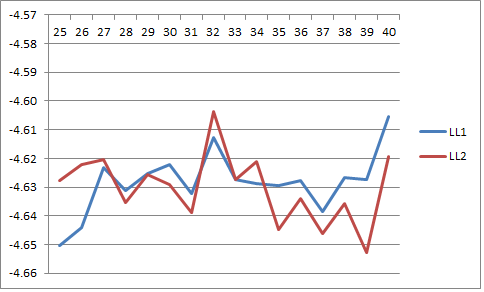
\includegraphics[scale=1.0]{LL-over-m-copy.png}}

\paragraph*{5.}
\subparagraph{(a)}
Yes, the neural network will try to maximize the log-likelihood of the training corpus by assigning weights such that the probabilities of the unseen words will be near-zero. 
\subparagraph{(b)}

Yes. If $w_t$ appears many times in the training set, the weights will be adjusted such that the signal into the output node for $w_t$ will be large in general. 

\paragraph*{6.}

\begin{itemize}
	\item \textbf{the choice of their class is good $<$END$>$ : } log-likelihood was $-4.33420672257$
	\item \textbf{the choice of there class is good $<$END$>$ : } log-likelihood was $-4.88568029646$
\end{itemize}






\end{document}
	% line of code telling latex that your document is ending. If you leave this out, you'll get an error